\chapter{Estudios del Cotransportador vSGLT}
\section{Introducci\'{o}n}
El presente estudio se ocupa de una prote\'{i}na encontrada en la membrana de la bacteria \textit{Vibrio Parahaemoliticus}. Pero antes de realizar dicho estudio es necesario responder las siguientes preguntas fundamentales: ?`qu\'{e} es una prote\'{i}na? ?`de qu\'{e} est\'{a} conformada una prote\'{i}na? ?`d\'{o}nde se encuentran las prote\'{i}nas? ?`cu\'{a}l es el papel que desempe\~{n}an las prote\'{i}nas en los seres vivos? ?`Cu\'{a}l es la forma de las prote\'{i}nas?.\\ \\

Una prote\'{i}na es un pol\'{i}mero (pol\'{i}- Muchas -mero: Partes) que est\'{a} formado por una gran cantidad de unidades del mismo tipo, estas unidades se conocen como amino\'{a}cidos. Espec\'{i}ficamente se dice que las prote\'{i}nas son polip\'{e}ptidos \footnote{P\'{e}ptido: Mol\'{e}cula formada por una cadena de varios amino\'{a}cidos mediante un enlace llamado pept\'{i}dico; normalmente se le dice pept\'{i}do a una cadena con menos de $20\sim30$  amino\'{a}cidos} que tienen m\'{a}s de 50 amino\'{a}cidos, haciendo que su peso molecular sea mayor a 5000 Da \cite{Kuchel}.\\

Un amino\'{a}cido es una mol\'{e}cula org\'{a}nica formada por un carbono llamado $\alpha$ alrededor del cual se encuentran los grupos funcionales carboxilo y amino, adem\'{a}s de un hidr\'{o}geno y un radical que le da la identidad a cada amino\'{a}cido, ver figura \ref{fig:amino}.\\
\begin{figure}[H]
\centering
\chemfig{C^{\alpha}(-[:0]H)(-[:90]COO^{-})(-[:180]NH_{3}^{+})(-[:270]R)}
\caption{Forma general de un L-amino\'{a}cido a pH 7. El radical \ce{R} cambia para cada amino\'{a}cido.}\label{fig:amino}
\end{figure}
A continuaci\'{o}n se muestran los 20 amino\'{a}cidos proteinog\'{e}nicos  comunes \footnote{Son los incorporados en la s\'{i}ntesis de prote\'{i}nas durante la traducci\'{o}n en el ribosoma}  clasificados de acuerdo a la carga, la polaridad y la formaci\'{o}n de grupos arom\'{a}ticos. Las abreviaciones de los amino\'{a}cidos se encuentran en la secci\'{o}n Lista de S\'{i}mbolos.\\
\begin{figure}[H]
\begin{center}
\begin{picture}(100,110)
\put(0,60){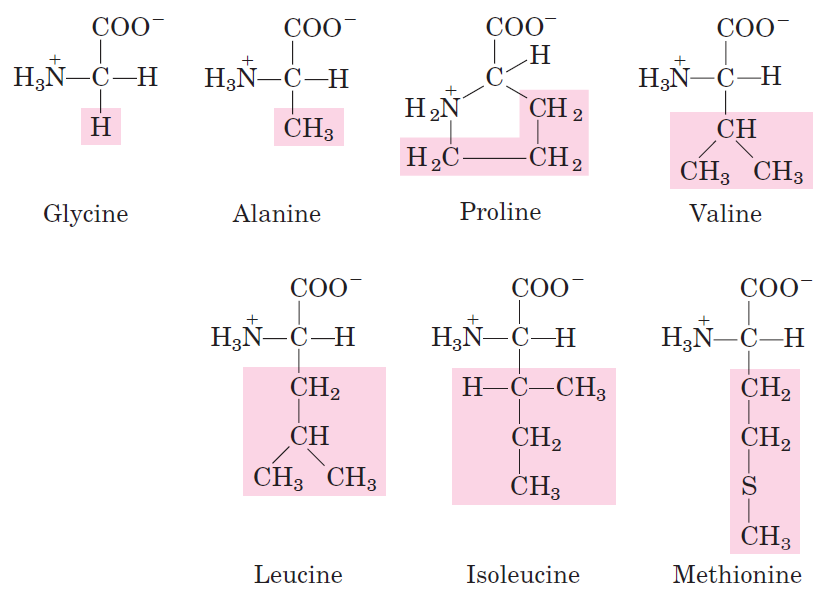
\includegraphics[scale=0.3]{Kap2/nopolar.png}}
\put(70,75){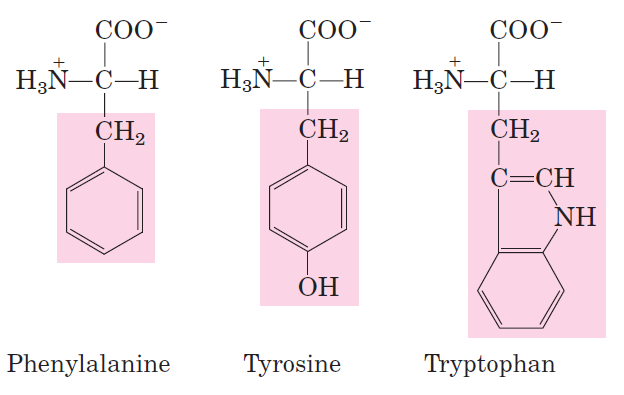
\includegraphics[scale=0.3]{Kap2/aromatico.png}}
\put(0,0){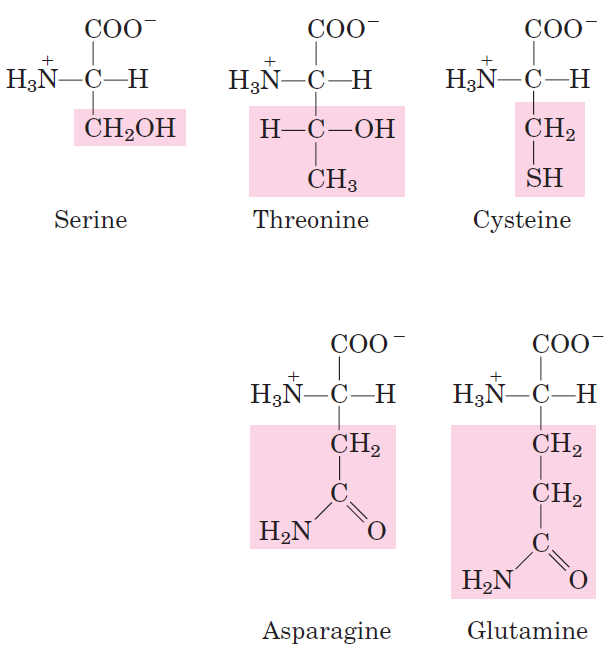
\includegraphics[scale=0.3]{Kap2/polardescargado.png}}
\put(70,30){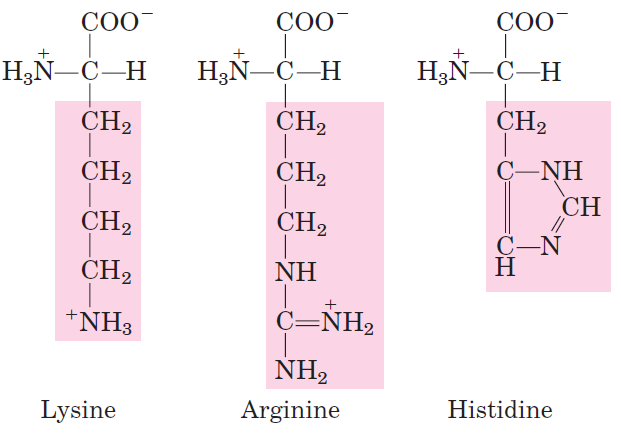
\includegraphics[scale=0.3]{Kap2/qpp.png}}
\put(70,-5){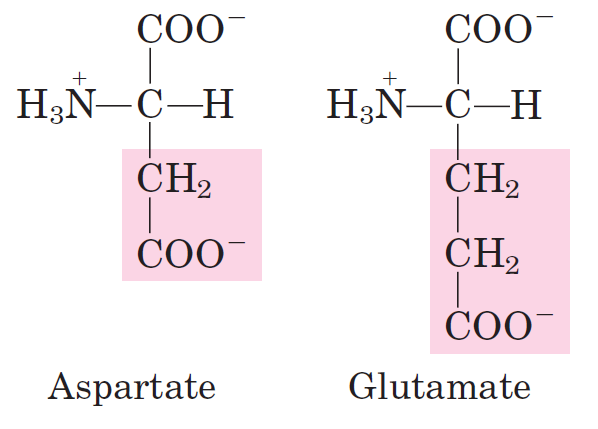
\includegraphics[scale=0.2]{Kap2/qmm.png}}
\put(0,110){No polar, grupo R alif\'{a}tico}
\put(70,110){Grupo R arom\'{a}tico}
\put(0,55){Polar descargado}
\put(70,65){Grupo R cargado positivamente}
\put(70,20){Grupo R cargado negativamente}
\end{picture}
\end{center}
\caption{F\'{o}rmulas estructurales de los 20 amino\'{a}cidos proteinog\'{e}nicos a pH 7 clasificados seg\'{u}n su radical de color rosado. Tomado de \cite{Nelson2011}.}
\end{figure}
Exceptuando la glicina, todos los amino\'{a}cidos presentan la propiedad de la quiralidad, existiendo dos posibles formas posibles para cada amino\'{a}cido: L-amino\'{a}cidos o D-amino\'{a}cidos. La distinci\'{o}n va seg\'{u}n la direcci\'{o}n en la que desv\'{i}en la luz con respecto al centro quiral que es el C-$\alpha$ del amino\'{a}cido.  Pr\'{a}cticamente todos los amino\'{a}cidos encontrados en prote\'{i}nas tienen la forma L.
\section{Formaci\'{o}n de P\'{e}ptidos y Prote\'{i}nas}
Dos amino\'{a}cidos reaccionan formando un enlace llamado pept\'{i}dico, esto ocurre cuando el carbono del grupo carboxilo se enlaza covalentemente con el nitr\'{o}geno del grupo amino produciendo una deshidrataci\'{o}n, es decir, liberando agua. En la figura \ref{fig:pepti} se muestran los reactantes y los productos de la reacci\'{o}n.
\begin{figure}[H]
\centering
\definesubmol\a{C^{\alpha}(-[:270]H)(-[:0]C(=[:270]O)(-[:0].\textcolor{blue}{OH}))(-[:180]NH_{2})(-[:90]R^{1})}
\definesubmol\b{C^{\alpha}(-[:270]H)(-[:0]C(=[:270]O)(-[:0]OH))(-[:180]N(-[:90]H)(-[:180].\textcolor{blue}{H}))(-[:90]R^{2})}
\definesubmol\c{C^{\alpha}(-[:90]R^{1})(-[:270]H)(-[:0]C(=[:270]O)(-[:0]N(-[:90]H)(-[:0]C^{\alpha}(-[:90]R^{2})(-[:270]H)(-[:0]COOH))))(-[:180]NH_{2})}
\schemestart
\chemfig[][scale=0.75]{!\a}\+\chemfig[][scale=0.75]{!\b}\schemestop
\schemestart\arrow{<=>[][\chemfig[scale=0.75]{H_{2}O}]} \schemestop
\chemfig[][scale=0.75]{!\c}
\caption{Formaci\'{o}n de un dip\'{e}ptido. Se muestran los reactantes sin ionizar para ejemplificar, en sus formas polii\'{o}nicas  se ioniza el amino-terminal y el carboxi-terminal}\label{fig:pepti}
\end{figure}
El enlace pept\'{i}dico es un enlace amida de la forma \ce{R^{1}C(O)NHR^{2}}. Debido a que las amidas forman una estructura de resonancia tal como se ilustra en la figura \ref{fig:amide}, el enlace pept\'{i}dico forma un enlace parcial doble. Este enlace parcial doble, como los caracter\'{i}sticos de las estructuras de resonancia, es un h\'{i}brido entre el enlace simple y el enlace doble. De hecho, Linus Pauling y Robert Corey \cite{Nelson2011}, encontraron que la longitud del enlace pept\'{i}dico era de $1.32\AA{}$ la cual es menor a la de un enlace \ce{C-N} simple ($1.49 \AA{}$) y mayor a la de un enlace doble covalente \ce{C=N} ($1.27\AA{}$). \\

\begin{figure}[H]
\centering
\definesubmol\a{-[:0,0.5]C(=[:90]\lewis{0:4:,O})(-[:0]\lewis{2:,N}(-[:270]H)(-[:0,0.5]))}
\definesubmol\b{-[:0,0.5]C(-[:90]\lewis{0:4:,O})(=[:0]\lewis{2:,N}(-[:270]H)(-[:0,0.5]))}
\definesubmol\c{-[:0,0.5]C(-[:90,,,,rddbond]O)(-[:0,,,,lddbond]N(-[:270]H)(-[:0,0.5]))}
\schemestart
\chemfig[][scale=0.75]{!\a}\arrow{<->}[0,0.75]\chemfig[][scale=0.75]{!\b}\schemestop
\schemestart\arrow{<->}[0,0.75] \schemestop
\chemfig[][scale=0.75]{!\c}
\caption{Posibles estructuras de Lewis de la ani\'{o}n amida \ce{[C(O)NH]^{-2}} que al mezclarlas producen el estado resonante.}\label{fig:amide}
\end{figure}
\subsection{Estructura de las Prote\'{i}nas}
De acuerdo a Kai Linderstr{\o}m-Lang, la estructura de las prote\'{i}nas puede considerarse en varios niveles, conocidos como estructuras \textit{primaria}, \textit{secundaria}, \textit{terciaria} y \textit{cuaternaria}. En lo que sigue se detallan cada uno de estos niveles.
\subsubsection{Estructura Primaria y Secundaria}
Por \textit{estructura primaria} se entiende la secuencia u orden en que se encuentran los residuos unidos por enlaces pept\'{i}dicos dentro de un p\'{e}ptido o prote\'{i}na. Generalmente se conoce primero por m\'{e}todos experimentales de clivaje, la secuencia de los residuos. Conocer la secuencia es fundamental ya que esta determina la estructura tridimensional.\\

En la figura \ref{fig:pepti} se observa un residuo contiguo al otro en forma horizontal, es decir en su estructura primaria. Sin embargo, al observar al p\'{e}ptido tridimensionalmente la cadena que se forma no es lineal. Esto se debe a interacciones no covalentes entre los \'{a}tomos que no necesariamente est\'{a}n conectados por el enlace pept\'{i}dico. Estas interacciones hacen que los grupos funcionales dentro del p\'{e}ptido se encuentren a \'{a}ngulos diferentes. Para estudiar la estructura tridimensional se describir\'{a}n inicialmente, los \'{a}ngulos de rotaci\'{o}n entre los residuos que componen al p\'{e}ptido o prote\'{i}na.\\

Linus Pauling y Robert Corey encontraron que el enlace pept\'{i}dico forma una estructura planar (r\'{i}gida) que contiene 4 \'{a}tomos enlazados alrededor del \ce{C-N}, la cual se presenta debido al enlace parcial doble, de tal manera que fija el \'{a}ngulo de rotaci\'{o}n del grupo \ce{C=O} con respecto al grupo \ce{N-H}. El \'{a}ngulo $\omega$ entre los dos grupos es, excepto cuando hay prolinas, de $180\textdegree$ (conformaci\'{o}n trans). En la figura \ref{fig:pepti2} se pueden observar los \textit{planos amida} de los residuos.\\ 
\begin{figure}[H]
\centering
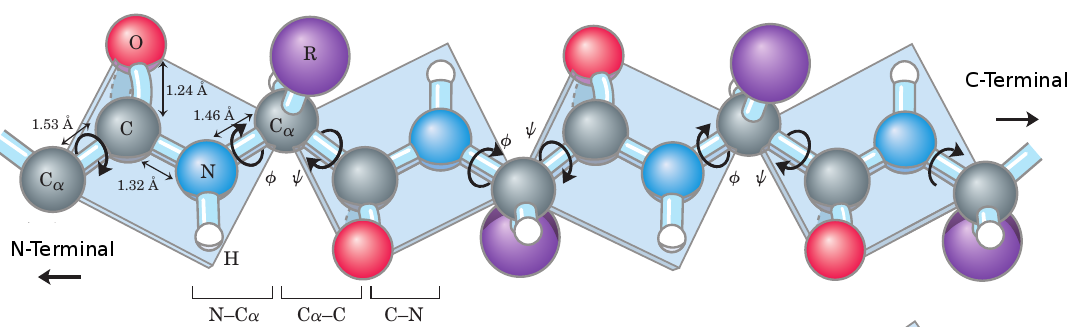
\includegraphics[scale=0.3]{Kap2/peptide.png}
\caption{\'{A}ngulos dihedros $\phi$, $\psi$ y $\omega$(No mostrado). Tomado de \cite{Nelson2011}.}\label{fig:pepti2}
\end{figure}
El \'{a}ngulo $\phi$ es $0\textdegree$ cuando el grupo \ce{N-H} est\'{a} en la posici\'{o}n trans respecto al enlace \ce{C\alpha-C} mientras que el \'{a}ngulo $\psi$ es  $0\textdegree$ cuando el enlace \ce{C-N} est\'{a} en la posici\'{o}n trans respecto al enlace \ce{C=O}, ver \cite{Kuchel}.\\

La \textit{estructura secundaria} se define como la conformaci\'{o}n local que genera estructuras repetitivas. Al definir la estructura secundaria se simplifica el entendimiento de la estructura tridimensional de la prote\'{i}na ya que permite identificar patrones que se repiten en diferentes prote\'{i}nas.\\

Existen tres tipos com\'{u}nes de estructura secundaria, ver \cite{Kuchel}:
\begin{enumerate}
 \item $\alpha$ H\'{e}lice: Ocurre si la cadena principal se enrolla formando una h\'{e}lice, de tal manera que el ox\'{i}geno del grupo carbonilo en un residuo forma un \textit{puente de hidr\'{o}geno} con el hidr\'{o}geno de la amina secundaria encontrado 4 residuos m\'{a}s adelante. En la figura \ref{fig:helice} se observan mediante las l\'{i}neas punteadas, \'{a}tomos de ox\'{i}geno (rojo) interactuando con los protones (gris claro)  en otro residuo. La cadena principal o esqueleto se representa con una cinta enrollada, figura de la izquierda cumpliendo la propiedad de tener 3.6 residuos por cada vuelta. Se observa que la secuencia en la h\'{e}lice avanza seg\'{u}n la regla de la mano derecha, esto es caracter\'{i}co de todas las h\'{e}lices formadas por L-amino\'{a}cidos, estas se les denomina $\alpha_R$ h\'{e}lices (Dextr\'{o}giras).
 \item Hoja plegada $\beta$ o l\'{a}mina $\beta$: Las hojas plegadas beta aparecen casi formando l\'{a}minas, contrario a la $\alpha$ h\'{e}lice. La hoja es formada por dos o m\'{a}s segmentos polipept\'{i}dos, contrario a la $\alpha$ h\'{e}lice, donde s\'{o}lo se requiere una cadena polipept\'{i}dica para formar la h\'{e}lice. Estos segmentos polipept\'{i}dicos est\'{a}n unidos por puentes de hidr\'{o}geno en los grupos carbonilo y amina de sus residuos. Hay dos tipos de l\'{a}minas $\beta$, las \textit{paralelas} que tienen sus cadenas polipept\'{i}dicas las mismas direccion\'{e}s, es decir del amino terminal al carboxi terminal o \textit{antiparalelas}, es decir, con direcciones opuestas entre s\'{i}. En la figura 
 \item Ovillos o Lazos Aleatorios: Son aquellos que no tienen una estructura secundaria repetitiva. En alguno
\end{enumerate}
\begin{figure}[H]
\centering
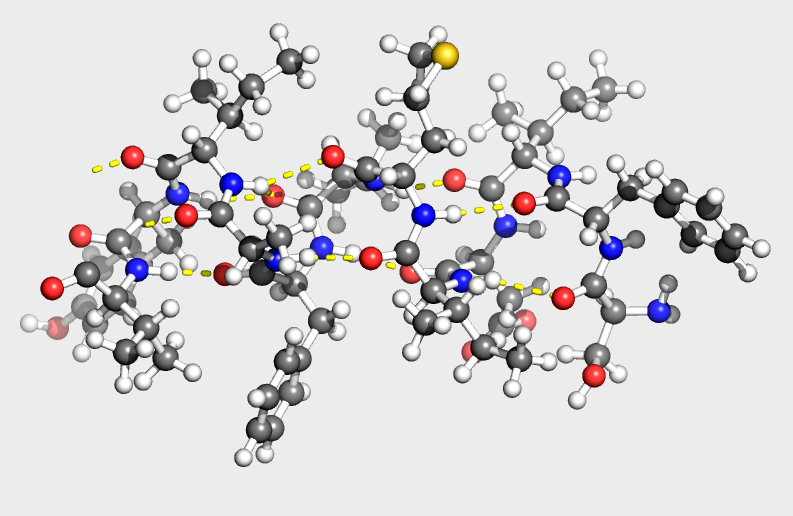
\includegraphics[scale=0.2]{Kap2/helix.png}
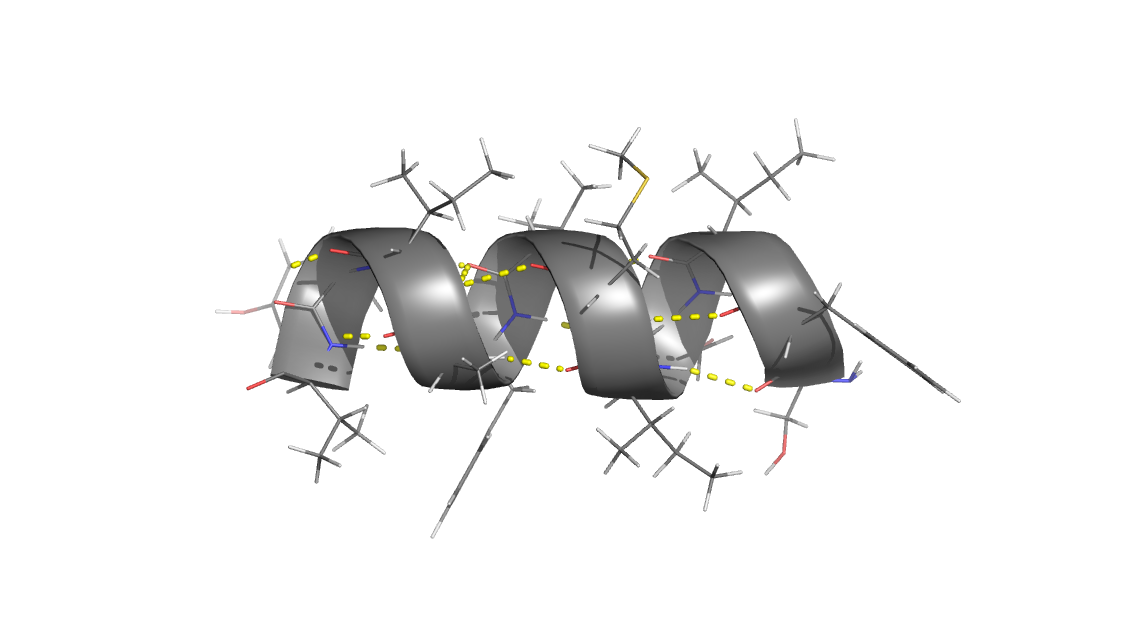
\includegraphics[scale=0.2]{Kap2/helix2.png}
\caption{Porci\'{o}n de una $\alpha$ h\'{e}lice perteneciente a la prote\'{i}na vSGLT (C\'{o}digo pdb 3DH4) formada por los enlaces de hidr\'{o}geno mostrados en color amarillo.}\label{fig:helice}
\end{figure}
\begin{figure}[H]
\centering
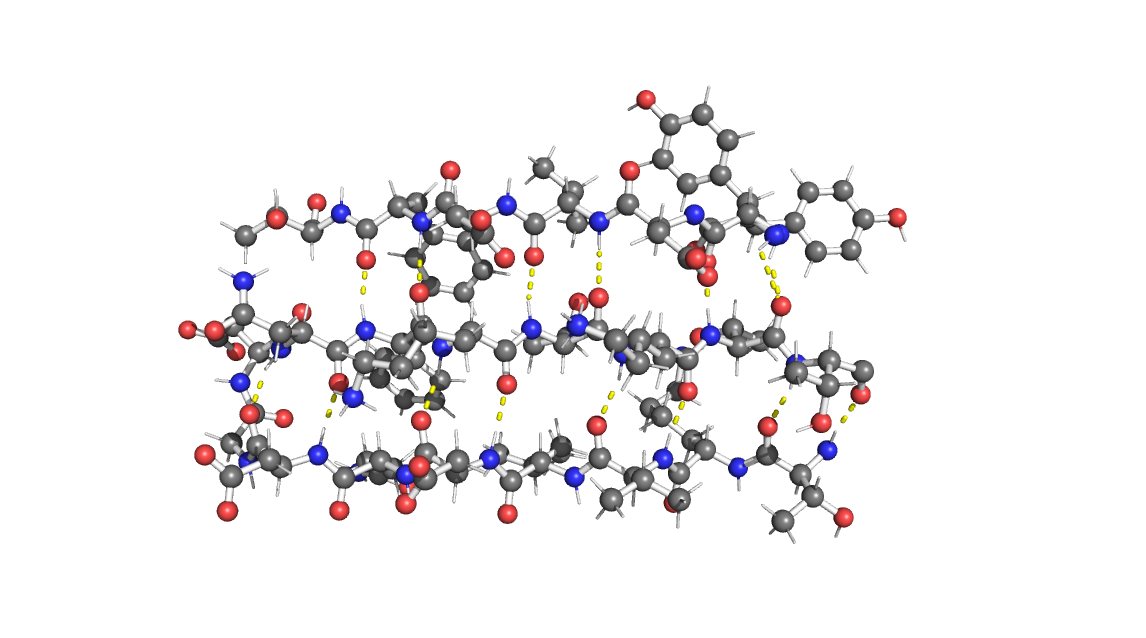
\includegraphics[scale=0.2]{Kap2/beta2.png}
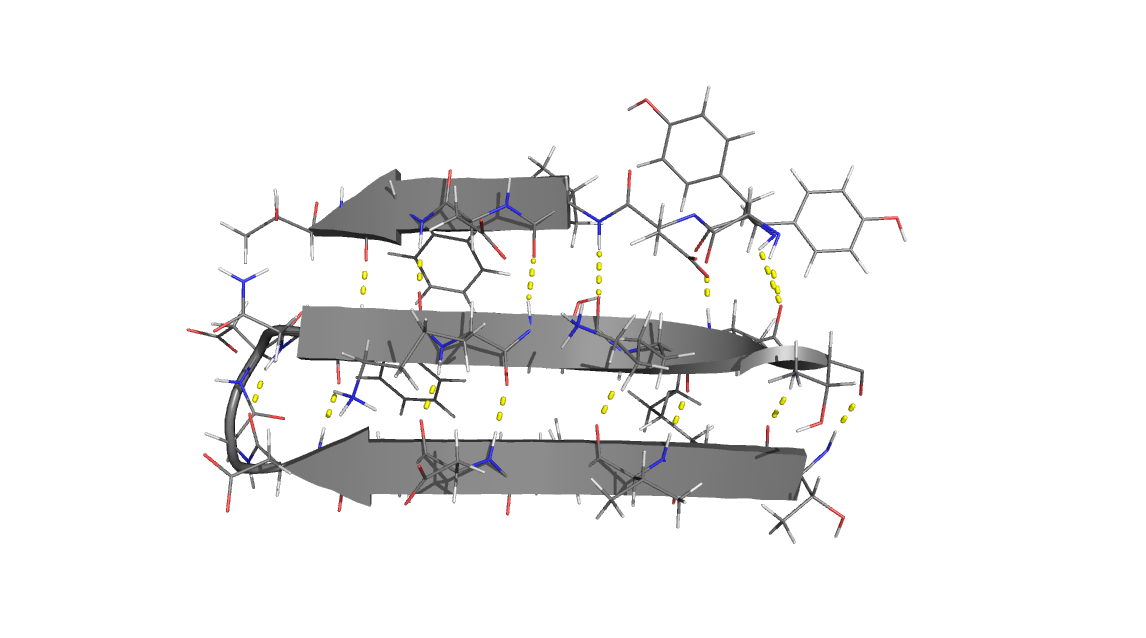
\includegraphics[scale=0.2]{Kap2/beta.png}
\caption{Porci\'{o}n de una hoja $\beta$ antiparalela perteneciente a la prote\'{i}na hRBP2 (C\'{o}digo pdb ) formada por los enlaces de hidr\'{o}geno mostrados en color amarillo.}\label{fig:beta}
\end{figure}
Tambi\'{e}n hay otros tipos de estructura secundaria como las h\'{e}lices de col\'{a}geno, las $\pi$ h\'{e}lices, las $3_{10}$ h\'{e}lices, entre otras, que no son de inter\'{e}s para estudiar nuestra prote\'{i}na.\\

Los patrones estructurales se forman cuando los \'{a}ngulos entre residuos son fijos. Precisamente esa es la diferencia entre una $\alpha$ h\'{e}lice y una hoja $\beta$, los \'{a}ngulos $\phi$ y $\psi$ entre residuos son diferentes. Aunque no hay \'{u}nicos \'{a}ngulos que determinen si conformaci\'{o}n es una $\alpha$ h\'{e}lice o una hoja $\beta$, al graficar $\psi$ contra $\phi$ , se han encontrado regiones permitidas y prohibidas para la formaci\'{o}n de estas conformaciones locales. El gr\'{a}fico de $\phi$ contra $\psi$ se conoce como gr\'{a}fico de Ramachandran. En la figura \ref{fig:Rama} se muestran las \'{a}ngulos permitidos en color oscuro para una $\alpha_R$ h\'{e}lice, una hoja $\beta$ y una $\alpha_L$ h\'{e}lice.
\begin{figure}[H]
\centering
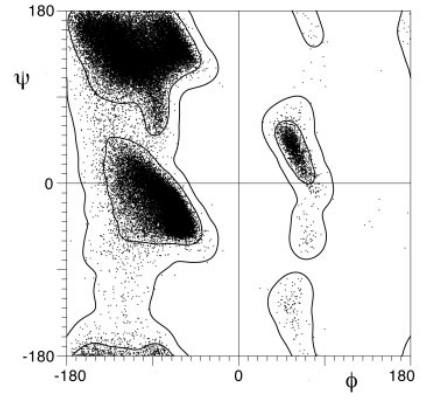
\includegraphics[scale=0.4]{Kap2/Rama.png}
\put(-33,30){$\alpha_R$}
\put(-16,35){$\alpha_L$}
\put(-30,50){$\beta$}
\caption{Gr\'{a}fico de Ramachandran para 97368 residuos tomados de 500 estructuras diferentes mostrando las regiones permitidas para una $\alpha_R$ h\'{e}lice, una $\alpha_L$ h\'{e}lice y una hoja $\beta$. Imagen tomada de \cite{Lovell2003}}\label{fig:Rama}
\end{figure}
\subsubsection{Estructura Terciaria}

\section{Prote\'{i}nas de Membrana}

\section{Transportadores}
La membrana celular al ser hidrof\'{o}bica permite protegerse de la regi\'{o}n extracelular, sin embargo, ella necesita ingresar y expulsar todos los compuestos necesarios para realizar su fisiolog\'{i}a OJO. La membranana celular tiene prote\'{i}nas que permiten el ingreso y la expulsi\'{o}n de estos compuestos. Entre los tipos de prote\'{i}nas se encuentran  los poros, las bombas, los transportadores y los canales. \\

Los transportadores se clasifican, de acuerdo al sistema de clasificaci\'{o}n de transportadores \cite{Nelson2011}, en dos categor\'{i}as principales de las cuales se desprenden otras subcategor\'{i}as :
\begin{enumerate}
 \item \textbf{Portadores}:
 \begin{enumerate}
 \item[1.] Transportadores activos primarios
 \item[2.a] Transportadores activos secundarios
  \begin{enumerate}
 \item[a)] Simportadores
 \item[b)] Antiportadores
 \end{enumerate}
 \item[2.b] Uniportadores
 \end{enumerate}
 \item  \textbf{Canales i\'{o}nicos}: Los canales se diferencian de los portadores en la raz\'{o}n a la que transportan los iones, que es de $10^6$ iones/segundo  (muy alta) as\'{i} como en que los canales no necesitan energ\'{i}a metab\'{o}lica para transportar los iones.
\end{enumerate}


Para visualizar las prote\'{i}nas se puede usar el microscopio de fuerza at\'{o}mico
\subsection{Cotransportadores}
Hacia la d\'{e}cada de los a\~{n}os sesenta Robert Crane, ver \cite{Hamilton2013}, estableci\'{o} una relaci\'{o}n acoplada o de \textit{cotransporte} entre el ion de sodio y la glucosa los cuales son absorbidos por el intestino delgado. El conocimiento de este mecanismo ha permitido realizar el tratamiento de la diarrea y del c\'{o}lera mediante la rehidrataci\'{o}n oral. La hip\'{o}tesis del cotransporte que ha sido numerosamente validada y ha sido una piedra angular para el entendimiento de el metabolismo de los carbohidratos, claves en la energ\'{e}tica celular. La hip\'{o}tesis del cotransporte tambi\'{e}n se ha extendido a otros organismos vivos, con la diferencia de que el acoplamiento del sodio se puede dar con cualquier otro soluto org\'{a}nico \cite{Faham2008}.\\
\section{Algunas Familias Proteicas y enrollamiento LeuT (LeuT fold)}
\section{Co-transportador vSGLT}
El cotransportador de Na+/Galactosa presente en la proteobacteria \textit{Vibrio Parahaemolyticus } denotado como vSGLT, es un simportador perteneciente a la familia de simportadores de $\mathrm{Na}^+$-soluto SSS \cite{SaierJr.quotTheFamilyquot}.\\
La caracterizaci\'{o}n molecular del compuesto se realiz\'{o} por primera vez hacia el a\~{n}o 2000 ver \cite{Turk2000}, mientras que la determinaci\'{o}n de su estructura fue posible hacia el a\~{n}o 2008 \cite{Faham2008}. En dichos estudios se establece que vSGLT es similar en la estructura primaria y terciaria a otros transportadores de la familia SLC5 como por ejemplo NIS, SGLT1, SGLT2.
\section{Estudios actuales del Co-transportador vSGLT}
